\section[The Significance of $\Delta t$]{\protect\boldmath The Significance of $\Delta t$}

\begin{overview}
\textbf{Overview:} The examples and activities in this section illustrate how the time duration $\Delta t$ of an impulse imparted on an object (or system) relates to the net force $\Sigma F$ and the change in momentum of the object (or system) $\Delta \vec{p}$.
\end{overview}

\subsection{The Tablecloth Trick}
\label{act7.1.3B}


\textbf{Phenomenon:} If a tablecloth (or a large piece of paper) is pulled quickly enough from under some objects sitting on it, those objects slide only a very short distance on the table top after the tablecloth has been pulled out from under them. This implies that they acquired only a small velocity from the tablecloth moving out from under them. If the tablecloth is pulled a little less quickly, the objects slide a little further on the table top, implying they acquired a slightly greater velocity.\\

\noindent\textbf{Try the trick:} Use a ``hanging mass'' or another object and a fairly large piece of paper. Try pulling the piece of paper at different rates, so that the object
	\begin{itemize}
		\item moves a lot (but does not fall off the table); and
		\item moves very little.
	\end{itemize}

\noindent In both cases, make sure you are pulling sufficiently fast so that the objects are continually sliding on the paper as it is being pulled. That is, you need to pull sufficiently fast so that the objects do not move with the paper.\\
	
\noindent\textbf{Our goal is to make sense of this phenomenon using the relation of impulse to a force and the time interval over which it acts.}

\subsubsection*{Establishing which part of the phenomenon we need to focus on:}
\note{For Activity~\ref{act7.1.3B} (\about\unit[70]{min?})}{
Make sure you practice this yourself so you know what it is about.  

1)  See below for discussion.


Below is an example of a complete Momentum Chart

Begin the solution by focusing on one object.  The initial time is before the pull and the final time is immediately after the cloth is no longer under the object.  Thus, the final momentum refers to the speed of the object just as the impulse goes to zero, but before it begins to slow down due to the impulse exerted by the tabletop.
\begin{center}
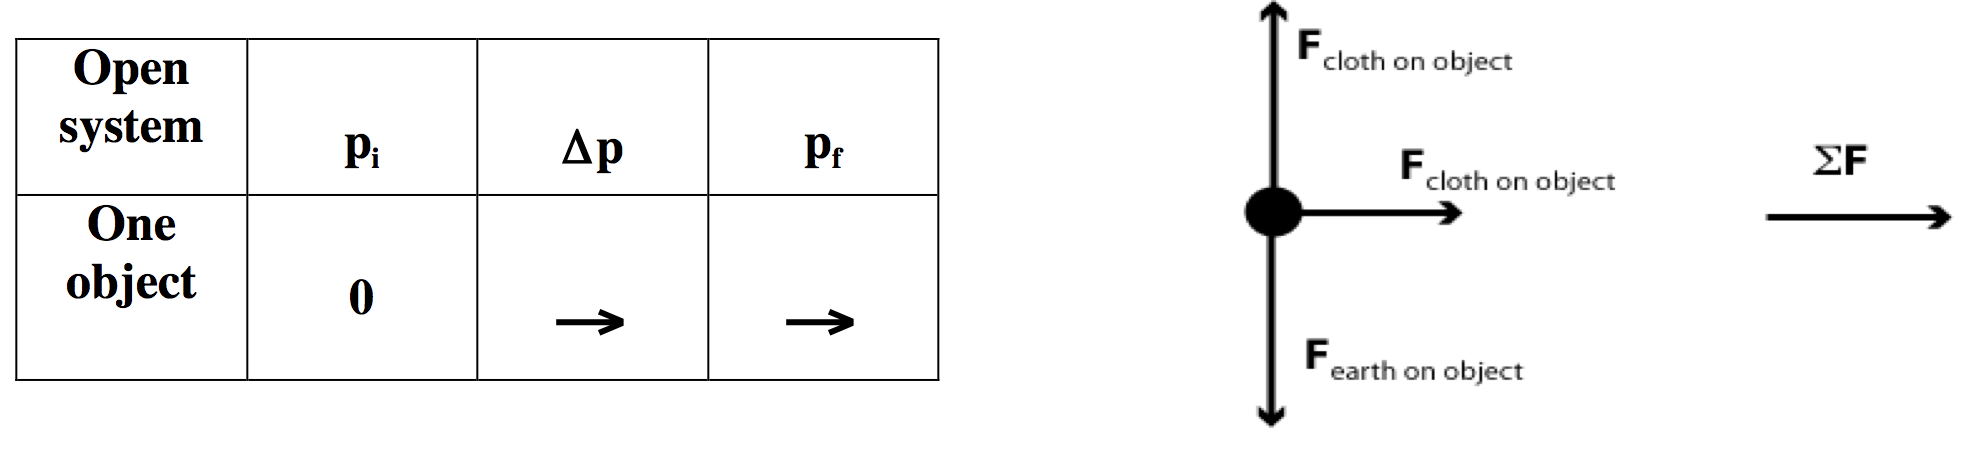
\includegraphics[width=.6\textwidth]{U7/figs/tableclothmomentumchart.png}
\end{center}

For object:  $\Delta \vec{p} = \vec{J} $ ,     $\vec{p}_{i}+\Delta \vec{p}= \vec{p}_{f}$\\
	$\vec{J} = \Sigma \vec{F} \Delta t = \mu m g \Delta t$,      $\vec{p} = m \vec{v}$ \\
	Since $p_{o} = 0$,    $p_{f} = \Delta \vec{p} = \vec{J} = \mu m g \Delta t = m v_{f}$
	Solving for $v_{f} $:    $ v_{f} = \mu g \Delta t$     \\Note that the mass of the object �drops out�, so all objects should have about the same speed due to the same cloth impulse.  Thus, they should all move about the same distance in coming to a rest on the tabletop.  Pulling faster gives a smaller final speed (and smaller stopping distance).  This should be reflected in the $\Delta \vec{p}$ column (longer for pulling slowly).

}
\begin{enumerate}
	\item The momentum of an object is first increased as the paper is pulled out from under it. Then the momentum is decreased back to zero as it slides to a stop on the table. How far it slides on the table after the paper is pulled out from under it is a qualitative measure of the speed it acquired when the paper was sliding under it: the greater the distance it slid, the greater the speed it had acquired.
	
	So, thinking in terms of impulse and momentum, \textbf{which force} acting through \textbf{what time interval} determined the maximum speed the object acquired before sliding to a stop on the table top?

\vspace{8pt}
\hspace{-\textwidth}\hspace{\linewidth} \textbf{Brief}
\hspace{\textwidth}\hspace{-\linewidth}
\WCD

	Express the friction force, which is the horizontal component of the force the paper exerts on the object, $F_{||\text{ paper on object}}$, as a constant (coefficient of friction $\mu$) times the object's weight $mg$.\footnote{Note that the coefficient will depend on the surfaces of the two materials in contact, but for reasonably smooth surfaces like paper and metal, it generally has a value in the range of 0.5 to 1.0.}
	
	\emph{The important point for the analysis here is that the \textbf{friction force} is \textbf{only proportional to the weight of the object} \boldmath$mg$. It does \emph{not} depend on how fast you pull the paper.}
	\note{2-5:}{The force of sliding friction, which is the net force acting on an object is something like 1/2 to 1 times the weight of the object for most combinations of typical surfaces.  That is, ?, the coefficient of sliding friction is typically between 0.5 and 1.0.  We tell students on this activity that sliding friction is the order of the weight, unless the surfaces are not smooth or special precautions have been taken to reduce friction.  Students should come away with the understanding that how fast (?t) you pull the tablecloth does NOT affect the net force on the object (Fnet = ?mg); it will make the impulse smaller the faster you pull (e.g., the faster you apply the force to get it moving from rest).}
	\item In your small group, make two complete \pcharts{} -- including force diagrams -- for one of the objects on your table (such as keys, small bottles, etc.) that is sitting on a piece of paper, which is pulled out from under it. One \pchart{} should show the process when the paper is pulled quickly, and the second \pchart{} should show the process when it is pulled less quickly. Consider the interval to be just before the pull until immediately after the paper is no longer under the object.
	
	\item Make sure all forces in the force diagrams are appropriately labeled. Does how fast you pull the tablecloth affect the net force acting on the object? Identify exactly what things are exerting forces on your object!
	
	\item Develop an explanation of these phenomena using the \pcharts{} you have prepared. Start by writing out an expression for impulse.
	
	\textbf{Extra question:} Try using different objects for your performance of the tablecloth trick. Do all the objects appear to move about the same distance for a given pull? How can you explain this?
	
	\item If you know the initial and the final momentum, you know the impulse. In each of your scenarios, did you have the same or a different impulse? So what is the effect of changing $\Delta t$? 
\end{enumerate}

\noindent Be prepared to explain what $\Delta t$ is and why it is important in a momentum problem!\\

\noindent Be ready to illustrate and give your explanations to the whole class.

\vspace{8pt}
\WCD